A harmonic function in one dimension is a homogeneous solution of the
partial differential equation with the Laplace operator
$\Delta = \partial^2/\partial x^2$ in one dimension.
Use the mean value property of $u$ to find the harmonic function
with $u(0)=0$ and $u(1)=1$.

\begin{loesung}
\begin{figure}
\centering
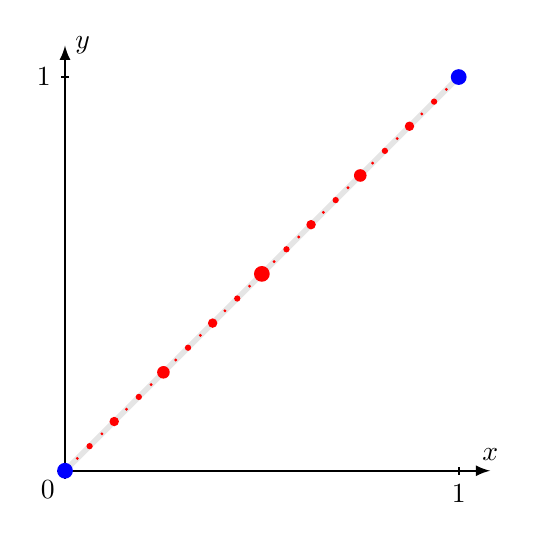
\begin{tikzpicture}[>=latex,thick]
\draw[color=gray!20,line width=2pt] (0,0) -- (5,5);
\draw[->] (-0.1,0) -- (5.4,0) coordinate[label={$x$}];
\draw[->] (0,-0.1) -- (0,5.4) coordinate[label={right:$y$}];
\draw (5,-0.05) -- (5,0.05);
\draw (-0.05,5) -- (0.05,5);
\node at (5,-0.05) [below] {$1$};
\node at (-0.05,5) [left] {$1$};
\node at (0,0) [below left] {$0$};
\fill[color=blue] (0,0) circle[radius=0.1];
\fill[color=red] (2.5,2.5) circle[radius=0.1];
\fill[color=blue] (5,5) circle[radius=0.1];
\foreach \x in {1,3}{
	\fill[color=red] ({5*\x/4},{5*\x/4}) circle[radius=0.08];
}
\foreach \x in {1,3,...,7}{
	\fill[color=red] ({5*\x/8},{5*\x/8}) circle[radius=0.06];
}
\foreach \x in {1,3,...,16}{
	\fill[color=red] ({5*\x/16},{5*\x/16}) circle[radius=0.04];
}
\foreach \x in {1,3,...,32}{
	\fill[color=red] ({5*\x/32},{5*\x/32}) circle[radius=0.02];
}
\end{tikzpicture}
\caption{Harmonic function in one dimension
\label{70000013:fig}}
\end{figure}
The mean value property means that the value in the middle of a
subinterval is the arithmetic mean of the values at the end points
of the interval.
In particular, $u(\frac12)=\frac12(u(0)+u(1)) = \frac12$.
Further subdividing the intervals obtained gives points
$(\frac14,\frac14)$ and
$(\frac34,\frac34)$ or more genereally
\[
\biggl(\frac{k}{2^n},\frac{k}{2^n}\biggr),
\qquad
\text{$n>0$ and $0\le k\le 2^n$,}
\]
giving all the rational points on the line $y=x$ with denominators that
are powers of $2$, suggesting that $y=x$ is the solution
(see figure~\ref{70000013:fig}).

In fact, the function $u(x)=x$ has the property that for any two
points $x_1$ and $x_2$, the value at $\frac12(x_1+x_2)$ ist
\[
u\bigl({\textstyle\frac12}(x_1+x_2)\bigr)
=
{\textstyle\frac12}(x_1+x_2)
=
\frac12\bigl(u(x_1) u(x_2)\bigr),
\]
so it satisfies the mean value property.
\end{loesung}

